\documentclass[journal,12pt,twocolumn]{IEEEtran}
\usepackage{graphicx}
\graphicspath{{./figs/}}{}
\usepackage{amsmath,amssymb,amsfonts,amsthm}
\newcommand{\myvec}[1]{\ensuremath{\begin{pmatrix}#1\end{pmatrix}}}
\usepackage{listings}
\usepackage{watermark}
\usepackage{titlesec}
\let\vec\mathbf
\lstset{
frame=single, 
breaklines=true,
columns=fullflexible
}

\title{\mytitle}
\title{
Matrix Assignment - Lines
}
\author{Pratheek Darla}
\date{October 2022}

\begin{document}
\maketitle
\tableofcontents
\bigskip


\section{\textbf{Problem}}
Find the orthocenter of the triangle formed by the lines xy =0
and x+y=1\\


\section{\textbf{Solution}}
Orthocenter of a triangle is the point where perpendiculars drawn to the opposite side from each vertex of the triangle intersect.   \\
\\
To find the orthocenter, first we find the coordinates of the vertices formed by the given lines xy = 0 and x+y = 1\\

Given lines x=0, y=0 and x+y=1 can be written as\\
\begin{equation}
\vec{n_1^{\top}} \vec{x} = c_1    \label{eq-1}
\end{equation}
\begin{equation}
\vec{n_2^{\top}} \vec{x} = c_2    \label{eq-2}
\end{equation}
\begin{equation}
\vec{n_3^{\top}} \vec{x} = c_3    \label{eq-3}
\end{equation}

where \begin{equation}	
	\vec{n_1} = \myvec{0 \\ 1}
	, \vec{n_2} = \myvec{1 \\ 0}, \vec{n_3} = \myvec{1 \\ 1},
\end{equation}
\begin{equation}
c_1=c_2=0 \quad and \quad c_3=1
\end{equation}
\\
By solving for equations ({\ref{eq-1}), (\ref{eq-2}) we get
\begin{equation}
\begin{pmatrix}
\vec{n_1^{\top}} \\
\vec{n_2^{\top}} 
\end{pmatrix} \vec{x_1} = \myvec{ c_1\\c_2}  \label{eq-6}
\end{equation}

\begin{equation}
\vec{x_1} = \begin{pmatrix}
\vec{n_1^{\top}} \\
\vec{n_2^{\top}} 
\end{pmatrix}^{-1}  \myvec{ c_1\\c_2}  \label{eq-7}
\end{equation}
\\
By substituting the values, we get
\begin{equation}
\vec{x_1} = \begin{pmatrix}
0 & 1 \\
1 & 0 
\end{pmatrix}^{-1}  \myvec{ 0\\0}  \label{eq-8}
\end{equation}
\\
By solving, we get
\begin{equation}
\vec{x_1} = \myvec{ 0\\0}  \label{eq-9}
\end{equation}
\\
Similarly, by solving ({\ref{eq-2}), (\ref{eq-3}) and ({\ref{eq-1}), (\ref{eq-3}) we get 
\begin{equation}
\vec{x_2} = \myvec{ 1\\0}  \label{eq-10},
\end{equation}

\begin{equation}
\vec{x_3} = \myvec{ 0\\1}  \label{eq-11}
\end{equation}
\\

So, the vertices of the triangle are \begin{equation*}
\vec{O} = \myvec{ 0 \\ 0}, \vec{A} = \myvec{ 1 \\ 0} \quad and \quad \vec{B} = \myvec{0 \\ 1}
\end{equation*}
	\\

The equation of line perpendicular to side AB is given by
\begin{equation}
	\vec{m_3^{\top}}(\vec{x}-\vec{O}) = 0   \label{eq-12}
\end{equation}
\\
where 
 $\vec{m_3} = \begin{pmatrix}
0 & 1 \\
-1 & 0 
\end{pmatrix}  \vec{n_3} = \myvec{ 1\\-1}$
\\

The equation of line perpendicular to side OB is given by
\begin{equation}
	\vec{m_1^{\top}}(\vec{x}-\vec{B}) = 0   \label{eq-13}
\end{equation}
\\
where 
 $\vec{m_1} = \begin{pmatrix}
0 & 1 \\
-1 & 0 
\end{pmatrix}  \vec{n_1} = \myvec{ 1\\0}$
\\

By solving for equations ({\ref{eq-12}), (\ref{eq-13}) we get
\begin{equation}
\begin{pmatrix}
\vec{m_3^{\top}} \\
\vec{m_1^{\top}} 
\end{pmatrix} \vec{x} = 
\begin{pmatrix}
\vec{m_3^{\top} O} \\
\vec{m_1^{\top} B}
\label{eq-14}
\end{pmatrix}
\end{equation}
\\
\begin{equation}
\vec{x} = \begin{pmatrix}
\vec{m_3^{\top}} \\
\vec{m_1^{\top}} 
\end{pmatrix}^{-1}  	
\begin{pmatrix}
\vec{m_3^{\top} O} \\
\vec{m_1^{\top} B}
\label{eq-14}
\end{pmatrix}
\end{equation}
\\
By substituting the values, we get
\begin{equation}
\vec{x} = \myvec{ 0\\0}  \label{eq-16}
\end{equation}
which is the Orthocenter of the triangle.

\section{\textbf{Figure}}
\begin{figure}[h]
    \centering
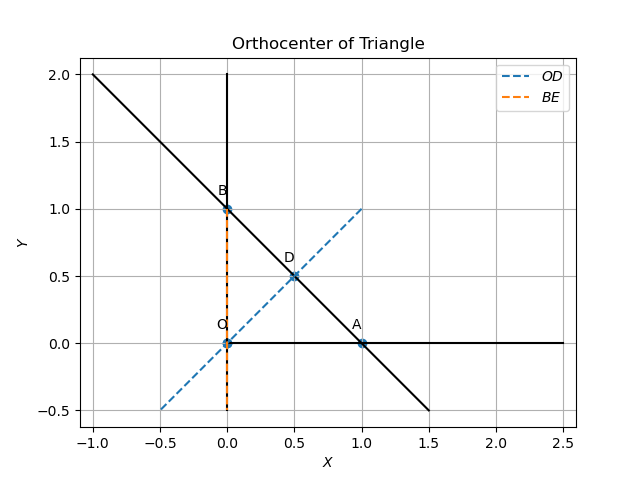
\includegraphics[width=\columnwidth]{fig2.png}
    \label{fig:my_label}
\end{figure}

\section{\textbf{Code Link}}

\begin{lstlisting}
https://github.com/PratheekDarla/FWC-IITH/blob/main/Matrix/Line/Assignment-line.py
\end{lstlisting}
Execute the code by using the command\\
\textbf{python3 Assignment-line.py}

\end{document}
